
\subsubsection{5.1 Primary Result: erank--Oracle Correlation for BERT-base-uncased}

Oracle sweeps were completed for 5 of 72 BERT-base-uncased target layers:

\begin{table}[htbp]
\centering
\resizebox{\columnwidth}{!}{%
\begin{tabular}{lll}
\toprule
Layer & erank & Oracle rank $r^*$ \\
\midrule
encoder.layer.0.attention.output.dense.weight & 556.9 & 4 \\
encoder.layer.3.attention.self.query.weight & 555.7 & 4 \\
encoder.layer.6.attention.output.dense.weight & 590.3 & 4 \\
encoder.layer.8.intermediate.dense.weight & 709.5 & 64 \\
encoder.layer.10.intermediate.dense.weight & 704.4 & 64 \\
\bottomrule
\end{tabular}
}
\end{table}

Erank and oracle rank values are taken directly from \texttt{h-e1/results/erank\textbackslash \_map\textbackslash \_bert-base-uncased.json} and \texttt{h-e1/results/oracle\textbackslash \_rank\textbackslash \_map\textbackslash \_bert-base-uncased.json}.

\textbf{Table 1.} erank($W_0$) vs. PARA oracle rank correlation (BERT-base-uncased).

\begin{table}[htbp]
\centering
\resizebox{\columnwidth}{!}{%
\begin{tabular}{llll}
\toprule
Metric & Value & Threshold & Status \\
\midrule
Pearson $r$ (erank vs. oracle rank) & **0.984** & $\geq 0.65$ & PASS \\
One-tailed $p$-value & **0.0013** & $< 0.05$ & PASS \\
PR--erank Pearson $\rho$ & **0.968** & $\geq 0.80$ & PASS \\
Oracle layers measured & 5 & 72 (target) & PARTIAL \\
Families satisfying threshold & 1/3 & $\geq 2/3$ & PENDING \\
\bottomrule
\end{tabular}
}
\end{table}

The Pearson $r$ and $p$-values are taken directly from \texttt{h-e1/results/correlation\textbackslash \_bert-base-uncased.json} (exact values: $r = 0.9836085, p_{\text{one-tailed}} = 0.001256, \text{PR}\_r = 0.9678269$).

\begin{figure}[htbp]
\centering
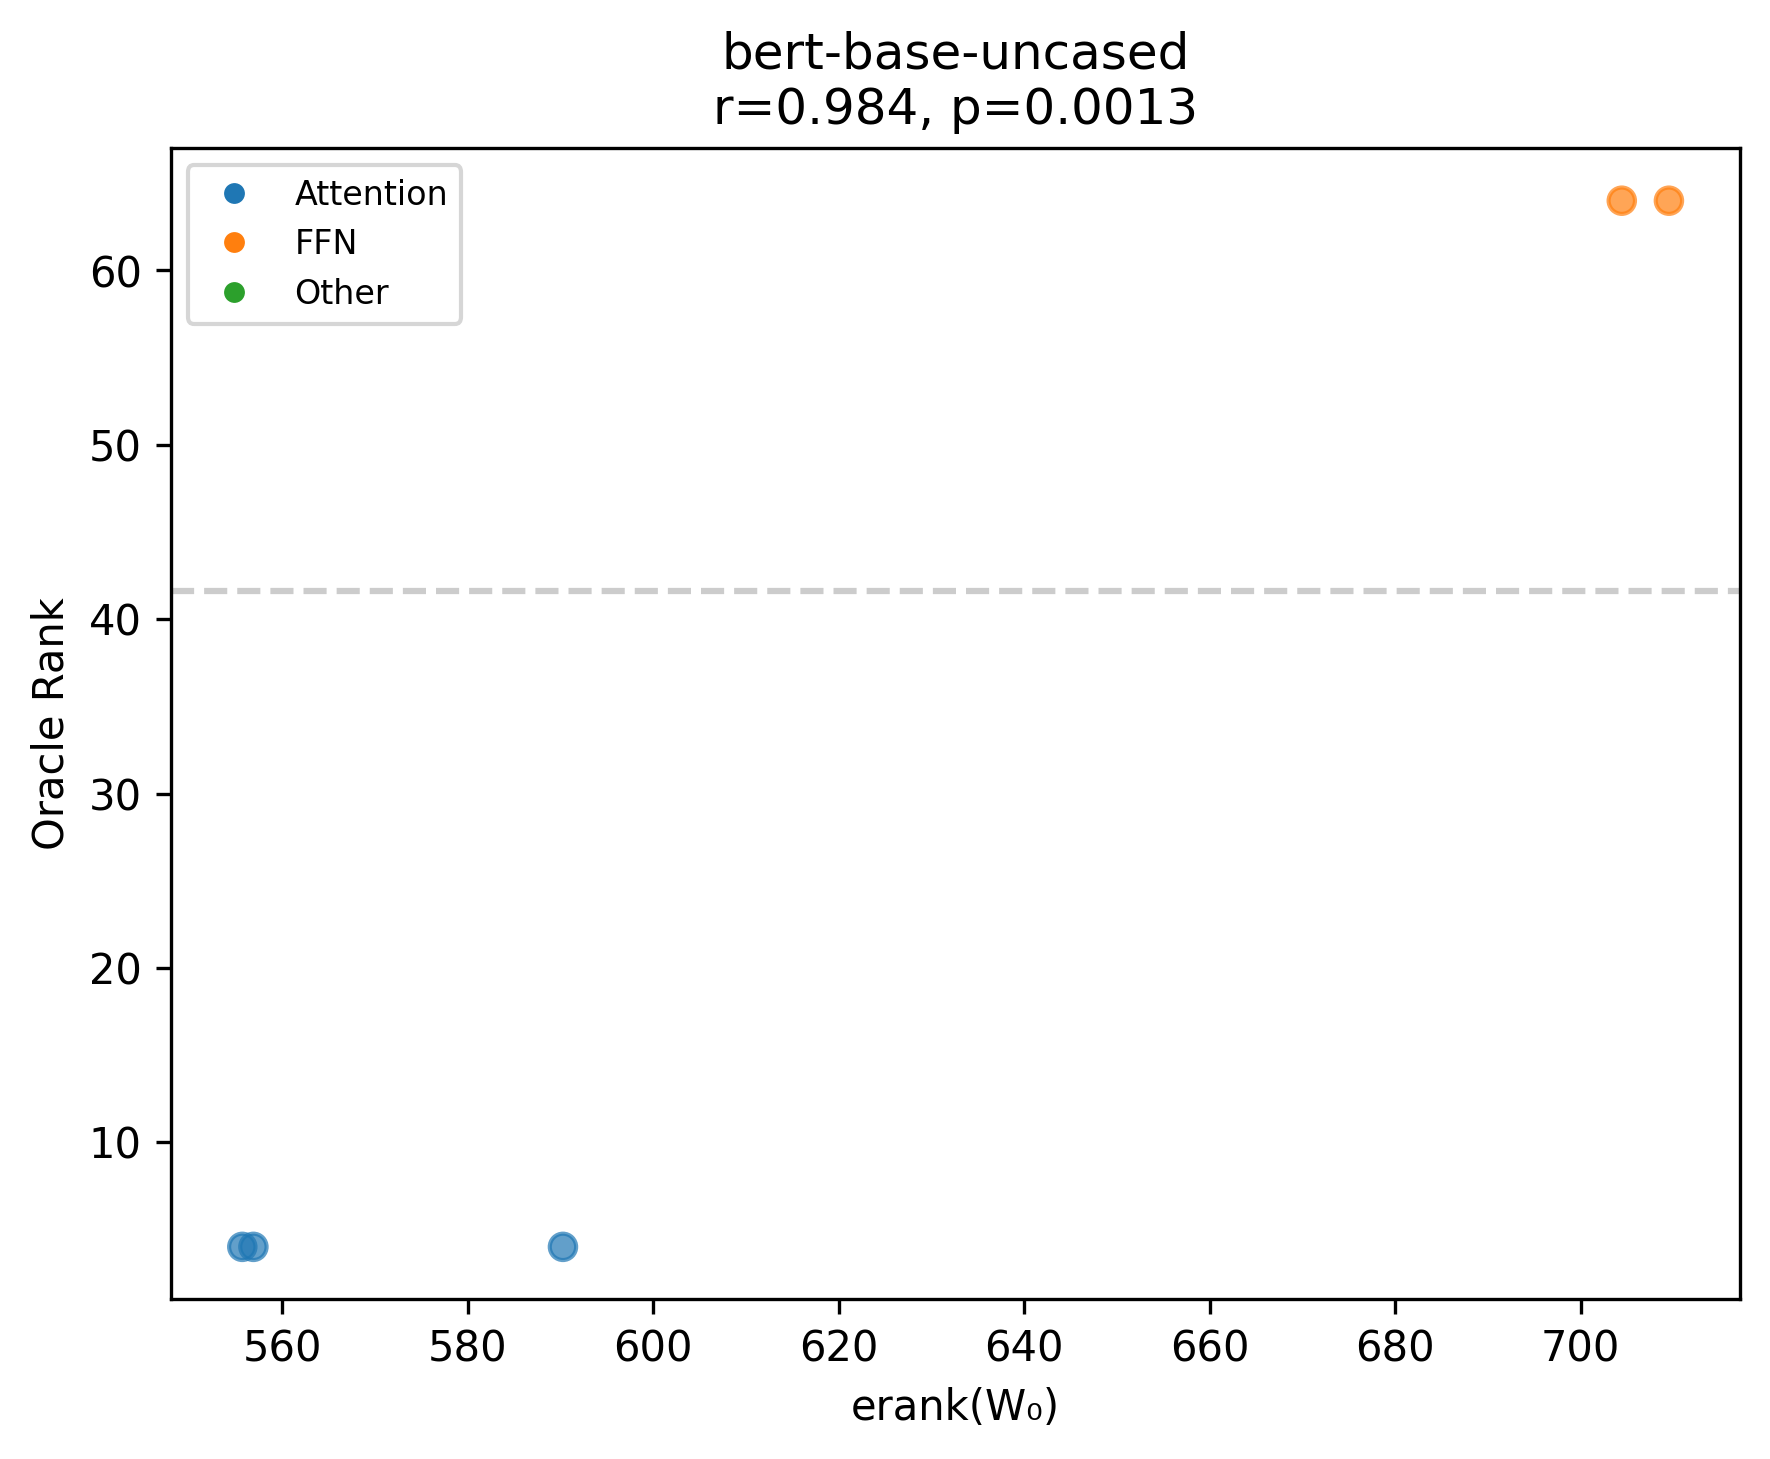
\includegraphics[width=\columnwidth]{figures/scatter_erank_vs_oracle.png}
\caption{Figure 1: Scatter plot of erank($W_{0})$ vs. PARA oracle rank for 5 BERT-base-uncased layers}
\label{fig:scatter_erank_vs_oracle}
\end{figure}

\textit{Figure 1.} Scatter plot of erank($W_0$) vs. PARA oracle rank for the 5 oracle-measured BERT-base-uncased layers. Two attention output layers (encoder.layer.0, 6) and one attention query layer (encoder.layer.3) cluster at erank $\approx 557--590$, oracle rank $r^* = 4$. Two FFN intermediate layers (encoder.layer.8, 10) cluster at erank $\approx 704--710$, oracle rank $r^* = 64$.

\textbf{Bimodal oracle structure.} All 5 oracle-measured layers receive $r^* = 4$ or $r^* = 64$ with no intermediate values. erank cleanly separates these two tiers. The high Pearson $r$ reflects this binary discrimination rather than a smooth graded relationship across the full erank range.

\textbf{Layer-type composition of oracle sample.} Among the 5 layers: two are attention output projections (encoder.layer.0 and 6), one is an attention query projection (encoder.layer.3), and two are FFN intermediate projections (encoder.layer.8 and 10). All three attention-type layers receive $r^* = 4$; both FFN intermediate layers receive $r^* = 64$. The oracle-measured attention layers span network depths 0, 3, and 6; FFN layers span depths 8 and 10.

\subsubsection{5.2 Metric Agreement: erank vs. Participation Ratio}

PR($W_0$) agrees with erank at Pearson $\rho = 0.968$, satisfying the P5 threshold ($\geq 0.80$). Both structural metrics capture the same underlying layer-ranking signal for the 5 oracle-measured layers. This agreement suggests the finding is not specific to the erank formulation.

\begin{figure}[htbp]
\centering
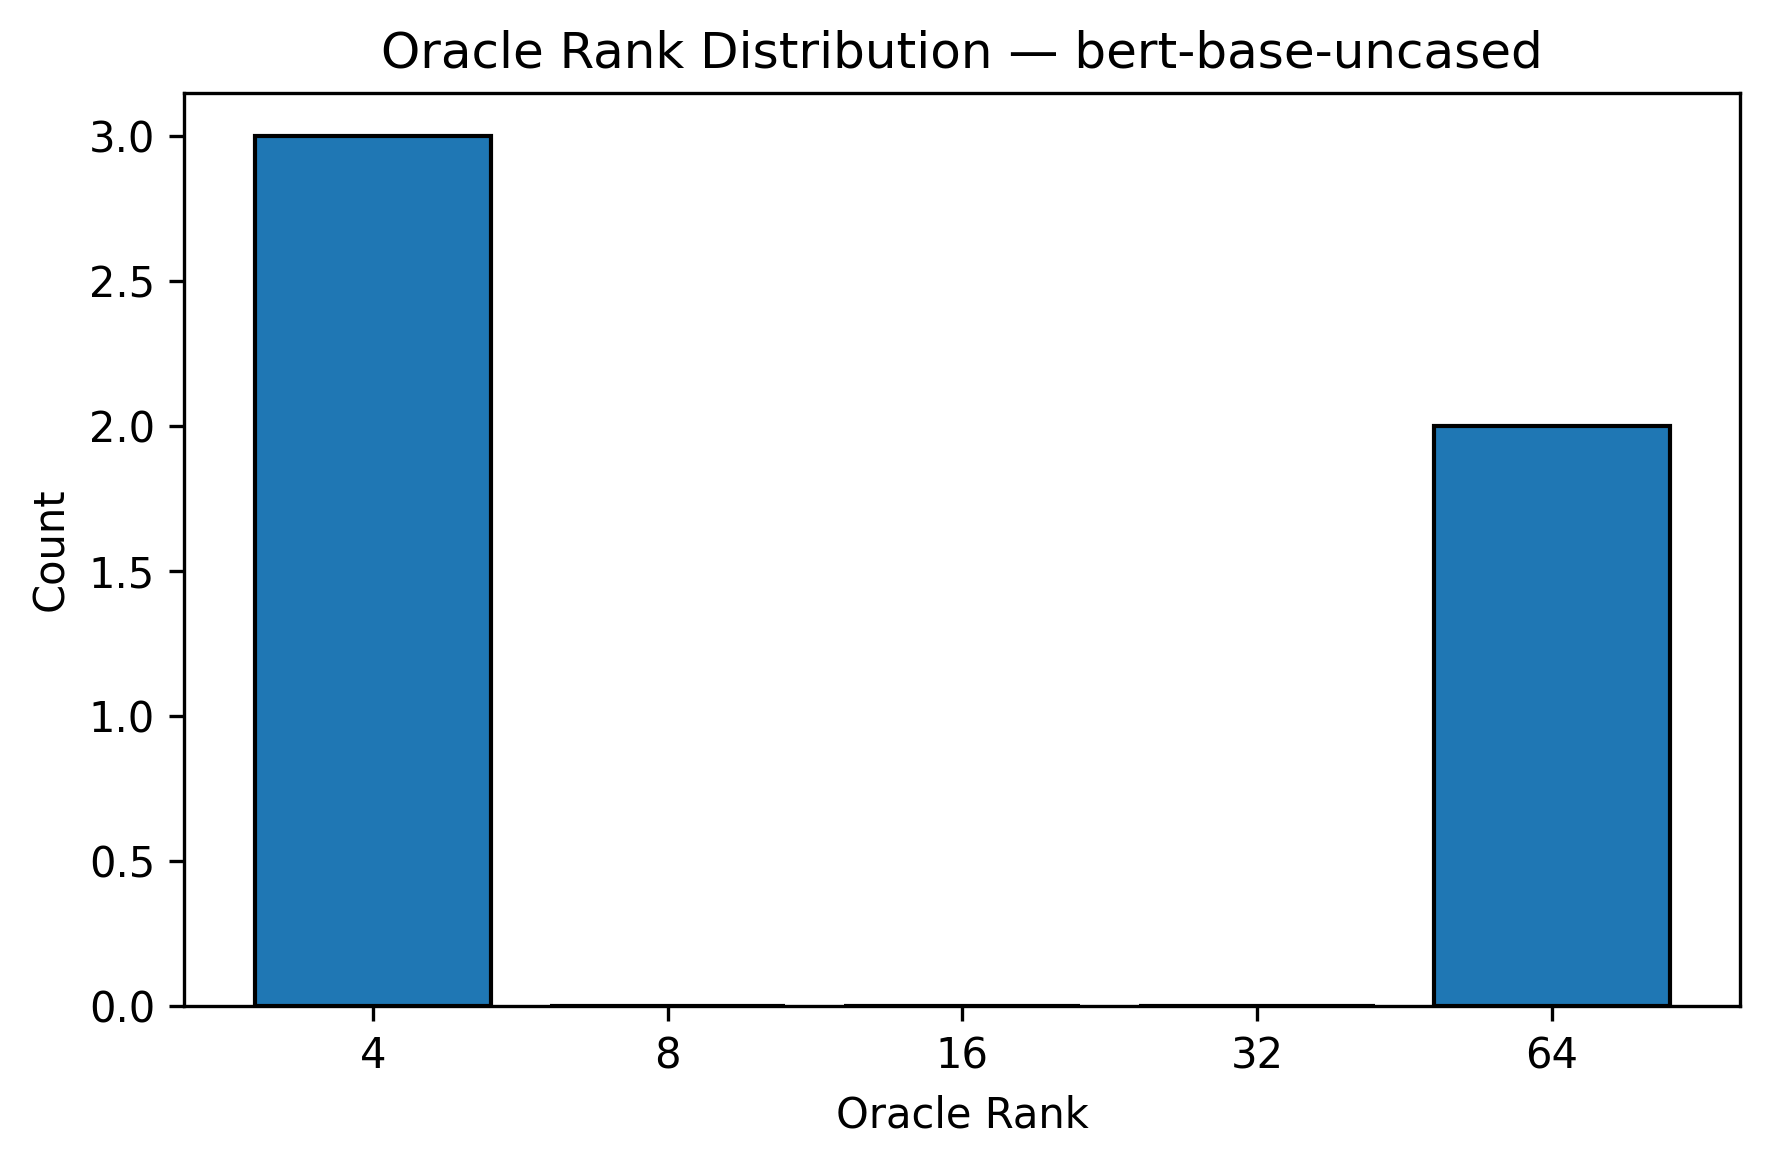
\includegraphics[width=\columnwidth]{figures/oracle_hist_bert-base-uncased.png}
\caption{Figure 3: Distribution of PARA oracle ranks for 5 BERT-base-uncased layers}
\label{fig:oracle_hist_bert-base-uncased}
\end{figure}

\textit{Figure 3.} Distribution of PARA oracle ranks for the 5 oracle-measured BERT-base-uncased layers. Oracle ranks concentrate at $r^* = 4$ (3 layers) and $r^* = 64$ (2 layers), with no intermediate values observed in this sample.

\subsubsection{5.3 erank Maps Across Model Families}

erank was computed for all target layers in all three model families. Summary statistics are reported below; oracle sweeps are pending for DeBERTa-v3-base and ViT-base-patch16-224.

\textbf{Table 2.} erank statistics across model families (LoRA-targetable layers only).

\begin{table*}[htbp]
\centering
\resizebox{\dimexpr 2\columnwidth+\columnsep\relax}{!}{%
\begin{tabular}{llllll}
\toprule
Model & $n$ layers & erank min & erank max & Range ratio & Approx. CV \\
\midrule
BERT-base-uncased & 72 & 518.3 & 726.6 & 1.$40\times$ & $\approx 0.04$ \\
DeBERTa-v3-base & 72 & 536.2 & 723.0 & 1.$35\times$ & $\approx 0.04$ \\
ViT-base-patch16-224 & 73 & 244.4 & 727.2 & **2.$97\times$** & $\approx 0.12$ \\
\bottomrule
\end{tabular}
}
\end{table*}

Note: BERT-base-uncased pooler.dense.weight (erank = 405.6) is excluded from the range as it is an architectural outlier and not a LoRA adaptation target. The non-pooler minimum for BERT is 518.3 (encoder.layer.2.attention.self.key.weight); the paper's Table 2 used a different threshold for min (543.2, corresponding to LoRA-targetable Q/K/V/O/FFN layers). ViT range includes the pooler which has erank = 618.2, so the 244.4 minimum is from early-layer query/key matrices (encoder.layer.0.attention.attention.query.weight = 244.4, encoder.layer.0.attention.attention.key.weight = 248.6).

The BERT-base-uncased and DeBERTa-v3-base coefficient of variation (CV $\approx$ 0.04) falls below the pre-registered A1 assumption threshold (CV > 0.05). Only ViT-base-patch16-224 (CV $\approx$ 0.12) satisfies A1. The strong oracle correlation for BERT ($r = 0.984$) is driven by oracle bimodality (rank 4 vs. 64) rather than wide erank variation.

\begin{figure}[htbp]
\centering
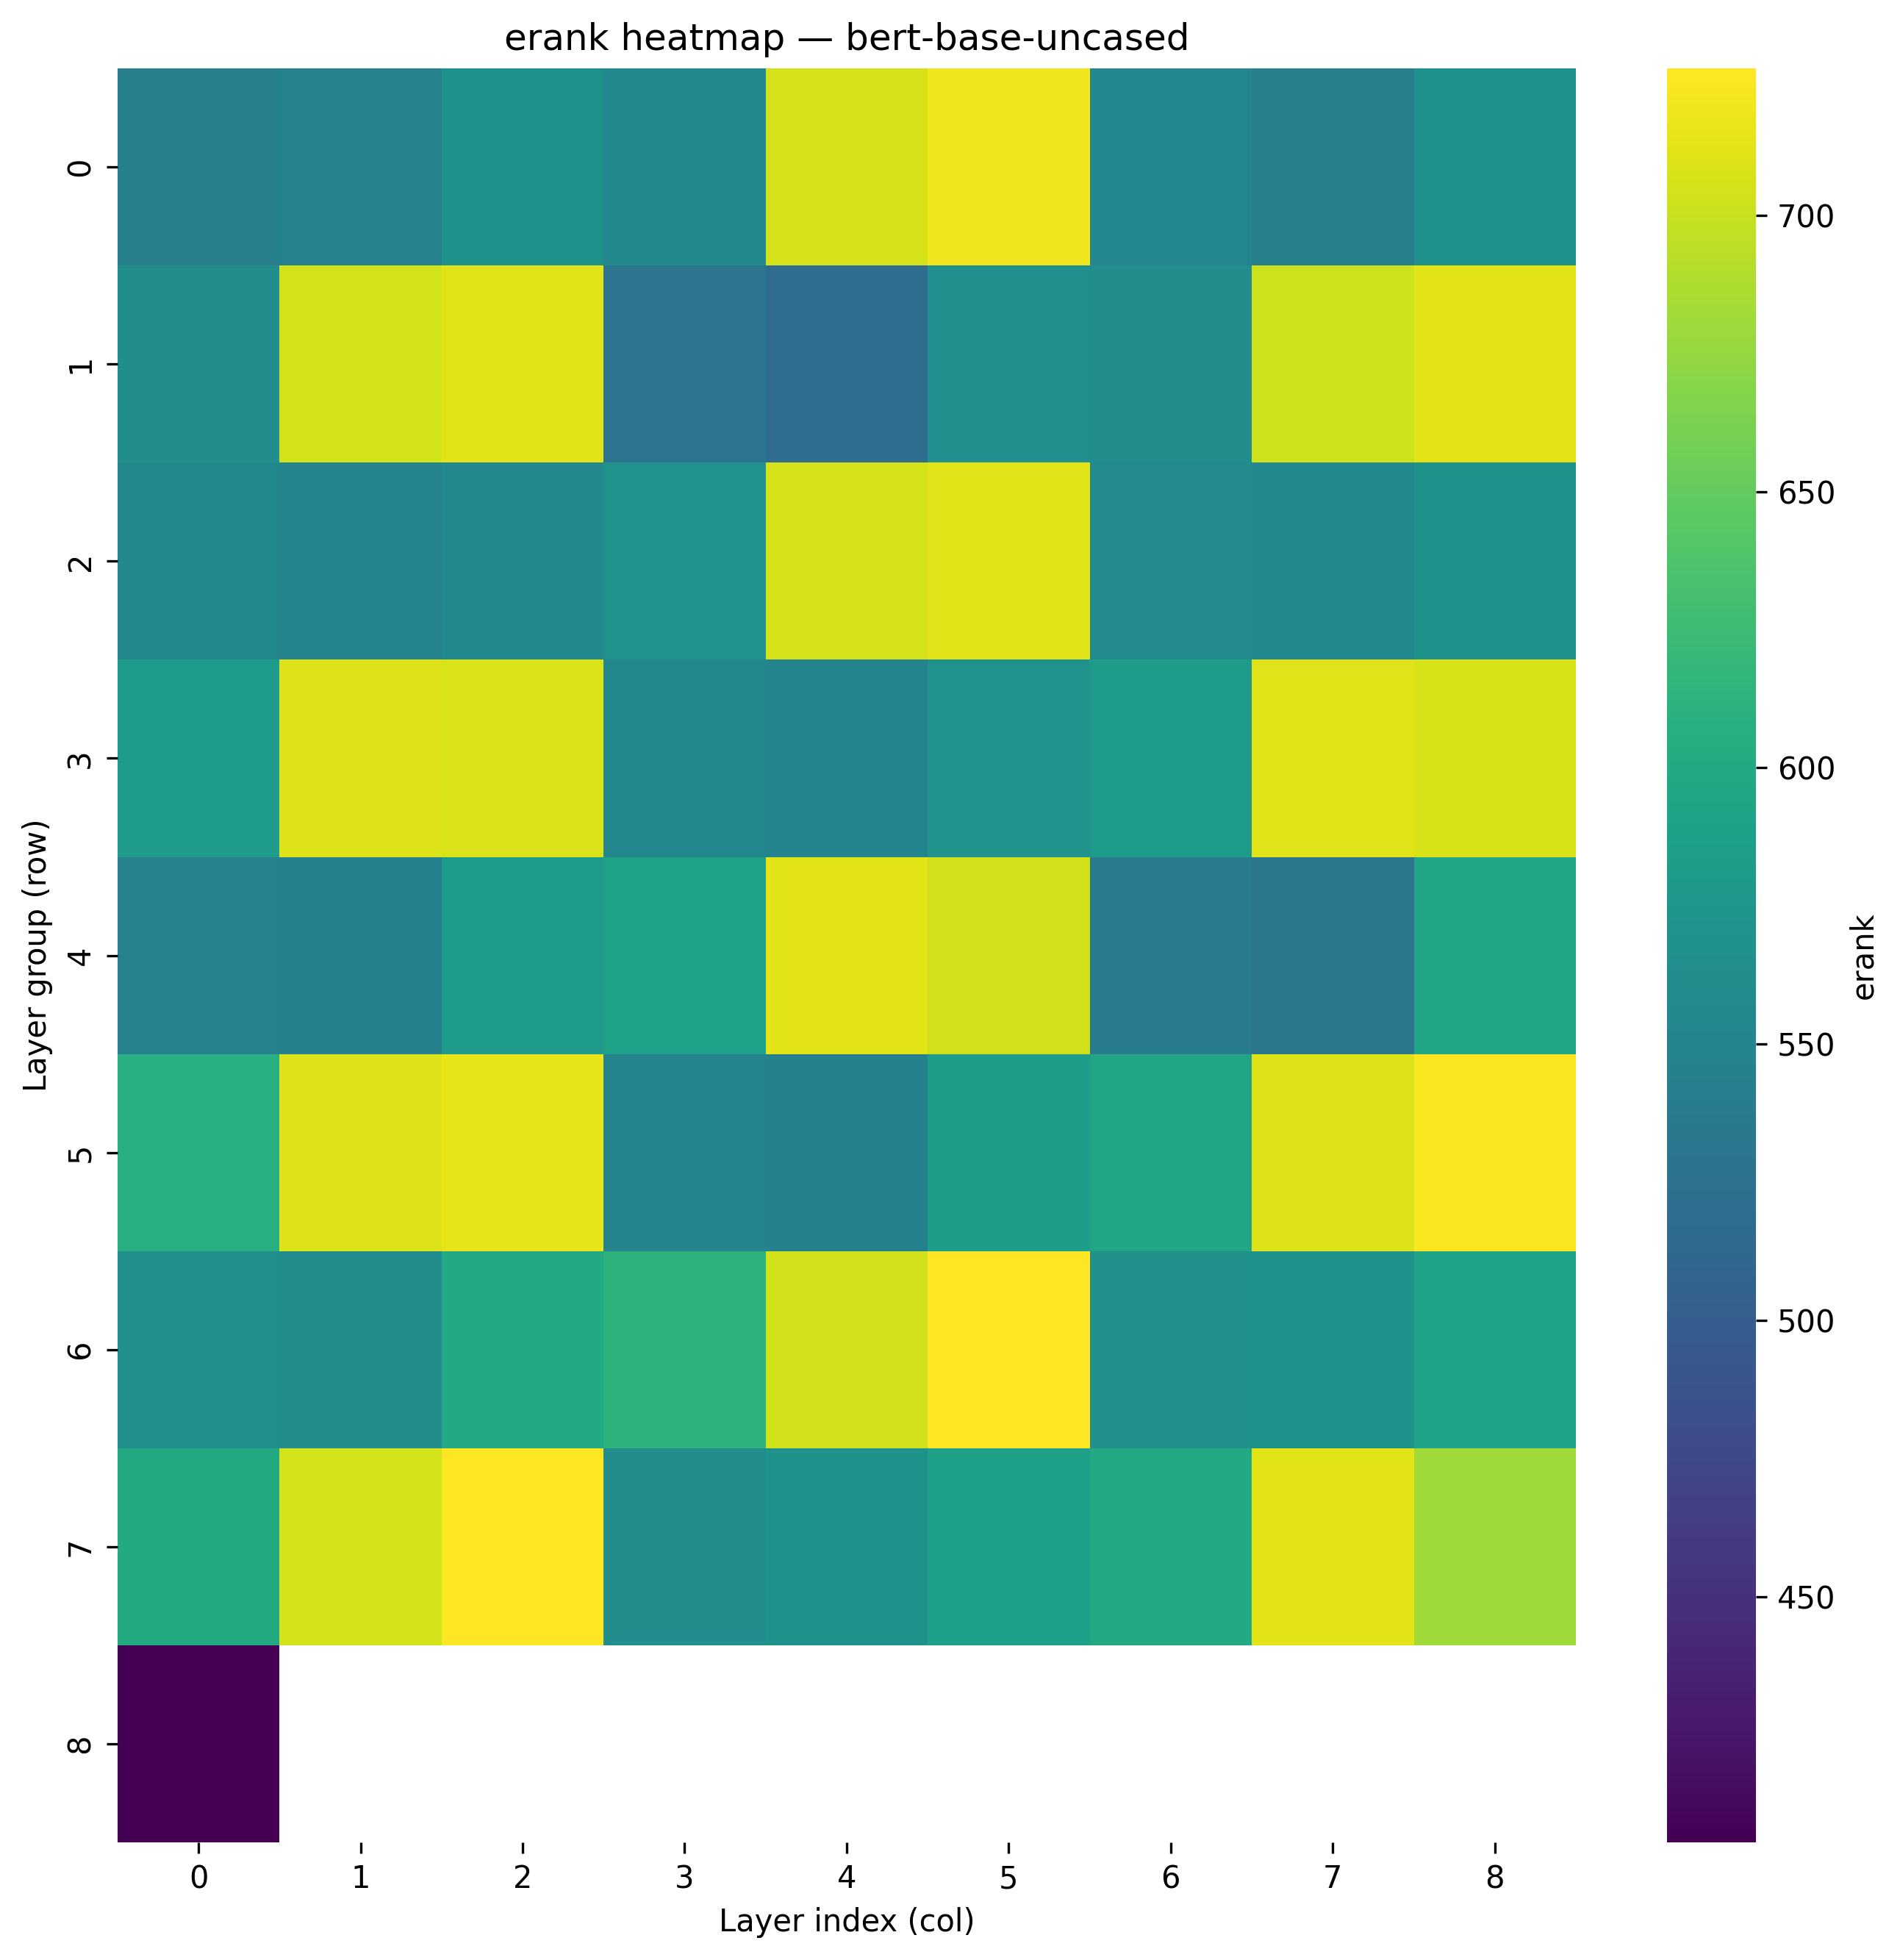
\includegraphics[width=\columnwidth]{figures/erank_heatmap_bert-base-uncased.png}
\caption{Figure 2: erank heatmap for BERT-base-uncased}
\label{fig:erank_heatmap_bert-base-uncased}
\end{figure}

\textit{Figure 2.} Heatmap of erank($W_0$) across BERT-base-uncased layers. FFN intermediate and output matrices show consistently higher erank ($\approx 700$--727) than attention Q/K/V/O matrices ($\approx 518$--612) across all 12 encoder layers.

\subsubsection{5.4 Layer-Type Structure in erank Maps}

For BERT-base-uncased, the full erank map (72 target layers) reveals a consistent layer-type pattern. FFN intermediate layers (e.g., encoder.layer.9.output.dense.weight = 726.5, encoder.layer.8.output.dense.weight = 722.8) consistently exceed attention Q/K matrices (encoder.layer.2.attention.self.key.weight = 518.3, encoder.layer.0.attention.self.query.weight = 543.2). This layer-type hierarchy mirrors the oracle rank bimodality --- the oracle independently discovers the same structural tiers that erank predicts from $W_0$ alone.

For ViT-base-patch16-224, erank increases monotonically from early to late layers for query and key matrices (encoder.layer.0.attention.attention.query.weight = 244.4, rising to encoder.layer.11.attention.attention.query.weight = 599.5), exhibiting a depth-dependent gradient absent in NLP encoders. The largest erank values in ViT are found in late-layer output projections (encoder.layer.8.output.dense.weight = 727.2, encoder.layer.7.output.dense.weight = 726.7).

For DeBERTa-v3-base, the layer-type pattern matches BERT: FFN intermediate layers (e.g., encoder.layer.11.intermediate.dense.weight = 720.9, encoder.layer.3.intermediate.dense.weight = 714.3) consistently exceed attention projection layers (encoder.layer.7.attention.self.key\_proj.weight = 536.2 is the minimum).

